\documentclass[letter,11pt]{article}
\usepackage{latexsym}
\usepackage{xcolor}
\usepackage{float}
\usepackage{amsthm}
\usepackage{amssymb}
\usepackage{wrapfig}
\usepackage{tabularx}
\usepackage{titlesec}
\usepackage{tikz}
\usepackage{geometry}
\usepackage{verbatim}
\usepackage{enumitem}
\usepackage{fancyhdr}
\usepackage{pgfornament}
\usepackage{multicol}
\usepackage{graphicx}
%\usepackage{cfr-lm}
\usepackage{booktabs}
\usepackage{svg}
\usepackage[T1]{fontenc}
\setlength{\multicolsep}{0pt} 
\pagestyle{fancy}
%\fancyhf{} % clear all header and footer fields
\fancyhead{}\fancyfoot{}
\fancyhead[R]{\textbf{\thepage}}
\fancyhead[L]{Aiden M. Rosenberg, MMXXIII A.D. }
\addtolength{\headwidth}{3cm}


\renewcommand{\headrulewidth}{1pt}
\renewcommand{\footrulewidth}{0pt}
\geometry{left=1.5cm, top=2.5cm, right=1.5cm, bottom=2cm}

%\usepackage{draftwatermark}	
%\SetWatermarkColor[gray]{0.9}
%\SetWatermarkText{Private}
%\SetWatermarkScale{3}

\usepackage[most]{tcolorbox}
\tcbset{
	frame code={}
	center title,
	left=0pt,
	right=0pt,
	top=0pt,
	bottom=0pt,
	colback=gray!20,
	colframe=white,
	width=\dimexpr\textwidth\relax,
	enlarge left by=-2mm,
	boxsep=4pt,
	arc=0pt,outer arc=0pt,
}


\raggedright
\setlength{\tabcolsep}{0in}

% Sections formatting
\titleformat{\section}{
  \vspace{-4pt}\scshape\raggedright\large
}{}{0em}{}[\color{black}\titlerule \vspace{-7pt}]

\begin{document}

\thispagestyle{empty}

\fontfamily{cmr}\selectfont
%----------HEADING-----------------

\parbox{2.35cm}{%
  \includesvg[width=2.3cm]{logo.svg}
}
\parbox{0.3cm}{\hspace{0.3cm}}
\parbox{\dimexpr\linewidth-5cm\relax}{
\setlength{\tabcolsep}{0.5em}
\def\arraystretch{1.25}
\begin{tabular}{@{}llll@{}}
\toprule
 \multicolumn{4}{c}
 {\hspace{-0.5em}\textbf{Assignment}: Worksheet \#1 (Vectors, Lines/Planes, Parametrizations, Polar)} \\ \midrule
\textbf{Name:}      & D. Aiden M. Rosenberg    & \textbf{Professor:}   & Dr. Alan v. Herrmann Ph.D        \\
\textbf{Course:}    & Calculus III        & \textbf{Date:}        & August 24th, 2023 A.D.   \\ \bottomrule
\end{tabular}
}
\vspace{1cm}
\section{Vector Operations}
Consider $\vec{a} = \langle 2,-1,0 \rangle$ and $\vec{b} = 2\hat{i} - \hat{k}$
\begin{enumerate}[label=\Alph*.]
    \item Find a unit vector in the opposite direction as $\vec{a}$
        \begin{enumerate}
            \item $|\vec{a}| = \sqrt{2^2+(-1)^2+0^0} = \sqrt{5}$
            \item $\hat{a} = \frac{\vec{a}}{|\vec{a}|} = \langle \frac{2}{\sqrt{5}}, \frac{-1}{\sqrt{5}}, 0 \rangle$
            \item $-\hat{a} = \langle -\frac{2}{\sqrt{5}}, \frac{1}{\sqrt{5}}, 0 \rangle = \boxed{\frac{2}{\sqrt{5}}\hat{i} + \frac{1}{\sqrt{5}}\hat{j}}$         
        \end{enumerate}
    \item Is the figure determined by $\vec{a}$ and $\vec{b}$ a rectangle or a parallelogram? Justify your answer.
    \begin{enumerate}
        \item $\vec{a} \cdot \vec{b} = \langle 2,-1,0\rangle \cdot \langle 2,0,-1\rangle = 2(2)-1(0)+0(-1) = 4$
        \item $|\vec{b}| = \sqrt{2^2+0^2+(-1)^2}=\sqrt{5}$
        \item $4 = |\vec{a}||\vec{b}| \cos(\theta) \Longrightarrow \frac{4}{5} = \cos \theta $
        \item If $ \underbrace{\vec{a} \cdot \vec{b} = 0 \Longrightarrow \theta = \frac{\pi}{2}}_{90^{\circ} \text{ interior angles of the figure i.e. rectangle}}$, since $ 4 \neq 0$ it is a parallelogram. 
    \end{enumerate}
    \item Find the area of the figure from part B.
    \begin{enumerate}
        \item \begin{align*} \vec{a} \times \vec{b} &= \left|\begin{matrix} \hat{i} & \hat{j} & \hat{k}\\ 2 & -1 & 0 \\ 2 & 0 & -1 \end{matrix} \right| = \hat{i} \left|\begin{matrix} -1 & 0 \\ 0 & -1\end{matrix} \right| - \hat{j} \left|\begin{matrix} 2 & 0 \\ 0 & -1\end{matrix} \right|+ \hat{k} \left|\begin{matrix} 2 & -1 \\ 2 & 0\end{matrix} \right|\\ &= \hat{i} - \hat{j}(-2)+\hat{k}(0-(-2))\\ &= \hat{i} + 2\hat{j}+ 2\hat{k}
        \end{align*}
        \item $\text{Area } = \sqrt{1^2+ 2^2+2^2} = 3$
    \end{enumerate}
    \item Verify that the cross product $\vec{a} \times \vec{b}$ is orthogonal to both vectors $\vec{a}$ and $\vec{b}$.
    \begin{enumerate}
        \item $a\cdot (a\times b)= \langle 2, -1, 0\rangle \cdot \langle 1,2,2\rangle = 2(1)-(2)+0 = 0$
        \item $b\cdot (a\times b)= \langle 2, 0, -1\rangle \cdot \langle 1,2,2\rangle = 2(1)+0 -2 = 0$
        \item Q.E.D.
    \end{enumerate}
\end{enumerate}

\section{Lines and Planes}
Consider the following lines:
$$L_{1}: x=3+t, y=3-2t, z=1+t$$
$$L_{2}: x=5+s, y=1-4s, z=1+3s$$
\begin{enumerate}[label=\Alph*.]
    \item  Show if the lines are parallel, intersecting, or skew. If the lines are intersecting, determine the point of intersection (Point $P$).
    \begin{enumerate}
        \item $3+t=5+s \Longrightarrow t=2+s$
        \item $3-2t=1-4s \Longrightarrow 2=2t-4s$
        \item $1+t=1+3s \Longrightarrow t=3s$
        \item $2+s=3s \Longrightarrow s=1 \Longrightarrow t=3$
        \item When $s=1$ and $t=3$ the lines share a point $P(6,-3,4)$
    \end{enumerate}
    \item Find an equation for the plane containing the given lines. Put your answer in $ax + by + cz = d$ format.
    \begin{enumerate}
        \item \begin{align*}\vec{h} &= \left|\begin{matrix} \hat{i} & \hat{j} & \hat{k} \\ 1 & -2 & 1 \\ 1 & -4 & 3 \end{matrix}\right| \\ &= \left|\begin{matrix} -2 & 1 \\ -4 & 3 \end{matrix}\right| \hat{i} -  \left|\begin{matrix} 1 & 1 \\ 1 & 3 \end{matrix}\right| \hat{j} +  \left|\begin{matrix} 1 & -2 \\ 1 & -4 \end{matrix}\right| \hat{k} \\ &= -2\hat{i} -2\hat{j}-2\hat{k} \end{align*}
        \item \begin{align*} 0 &=\langle-2,-2,-2\rangle \cdot \langle x-x_0,y-y_0,z-z_0\rangle\\ & = -2(x-6)-2(y+3)-2(z-4)\\ &= -2x-2y-2z +14 \end{align*}
        \item $7=x+y+wz$
    \end{enumerate}
    \item Sketch the part of the plane in the first octant labeling intercepts.
    \begin{center}
        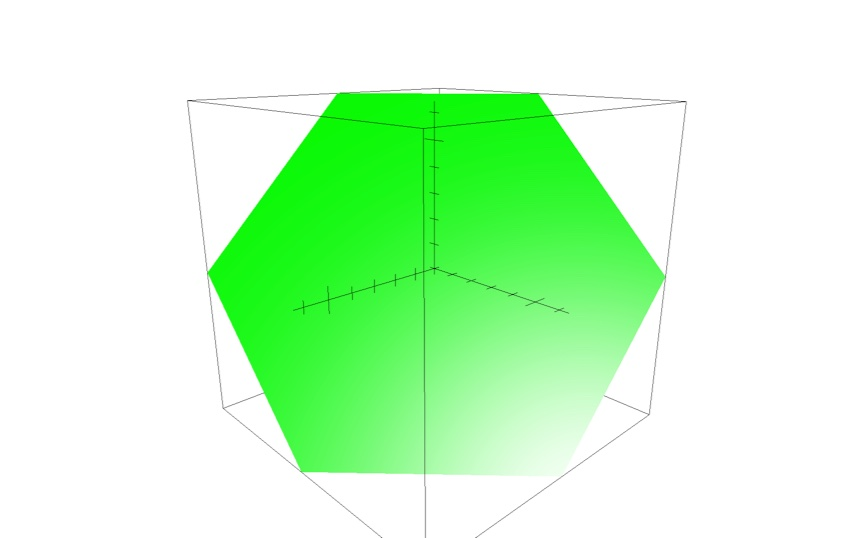
\includegraphics[width = 3in]{Graph 1.jpg}
    \end{center}
\end{enumerate}

\section{Parametrizations}
Find parametric equations for the following curves.

\begin{enumerate}[label=\Alph*.]
    \item Line segment from $P(8, -1, 9)$ to $Q(0, -4, 5)$
    \begin{enumerate}
        \item $\vec{\mathbf{r}}(t) = \mathbf{P}-t(\mathbf{Q}-\mathbf{P})$
        \item \begin{align*}\mathbf{r}(t) &= \begin{bmatrix} 8 \\ -1 \\ 9 \end{bmatrix} + t \left( \begin{bmatrix} 0 \\ -4 \\ 5 \end{bmatrix} - \begin{bmatrix} 8 \\ -1 \\ 9 \end{bmatrix} \right)\\ &=  \begin{bmatrix} 8 \\ -1 \\ 9 \end{bmatrix} + t \begin{bmatrix} -8 \\ -3 \\ -4 \end{bmatrix} \end{align*}
    \item When $0\leq t \leq 1$\begin{align*} x(t) &= 8 - 8t \\ y(t) &= -1 - 3t \\ z(t) &= 9 - 4t \end{align*}
    \end{enumerate}
    \item Section of parabola $y = -2x^2 + 10$ from $\underbrace{(1, 8)}_{t=0}$ to $\underbrace{(2, 2)}_{t=1}$
    \begin{enumerate}
        \item $x=t+a\rvert_{t=0} \Longrightarrow 1 = 0+a \Longrightarrow x = t+1$
        \item $y = -2(t+1)^2+10$
    \end{enumerate}
    \item Section of a circle of radius $2$, centered at the origin, traced out counterclockwise with initial point $(0, 2)$ and terminal point $(-2, 0)$.
    \begin{enumerate}
        \item $\frac{\pi}{2} \leq t \leq \pi$ \begin{align*}
            x = 2\cos t\\
            y=2\sin t
        \end{align*}
    \end{enumerate}
\end{enumerate}

\section{Polar Coordinates}
\begin{enumerate}[label=\Alph*.]
    \item Convert the point $(-2,2\sqrt{3})$ from rectangular to polar coordinates.
    \begin{enumerate}
        \item $r=\sqrt{(-2)^2 + \sqrt(2\sqrt{3})^2} = 4$
        \item \begin{align*}
            \theta &= \arctan\left(\frac{2\sqrt{3}}{-2}\right)\\
            &= \arctan\left(-\sqrt{3}\right)\\
            &= \frac{-\pi}{3}, \frac{2\pi}{3}
        \end{align*}
        \item \boxed{\left(4, \frac{2\pi}{3}\right)}
    \end{enumerate}
    \item Convert the point $\left(4,-\frac{\pi}{6}\right)$ from polar to rectangular coordinates.
    \begin{enumerate}
        \item $x=r\sin\theta \Longrightarrow x = 4 \underbrace{\sin\left(\frac{-\pi}{6}\right)}_{\frac{\sqrt{3}}{2}} = 2\sqrt{3}$ 
        \item $y=r\cos\theta \Longrightarrow x = 4 \underbrace{\sin\left(\frac{-\pi}{6}\right)}_{\frac{1}{2}} = -2$
        \item $$\boxed{(2\sqrt{3},2)}$$
    \end{enumerate}
    \item  Convert the polar equation $r = 4$ into a rectangular equation.
    \begin{enumerate}
        \item $ 4 = \sqrt{x^2+y^2} \Longrightarrow \boxed{x^2+y^2 = 16}$
    \end{enumerate}
    \item  Convert the rectangular equation $x^2 + (y-3)^2 = 9$ into a polar equation.
    \begin{enumerate}
        \item $(r\cos\theta)^2+ (r\sin\theta -3)^2 = 9$
        \item $r^2\cos^2\theta+r^2\sin^2\theta - 6r\sin\theta +9 = 9$
        \item $\cos^2 + \sin^2 = \frac{6\sin\theta}{r}$
        \item $1 = \frac{6\sin\theta}{r}$
        \item $r=6\sin\theta$
    \end{enumerate}
\end{enumerate}
\end{document}
